% This is samplepaper.tex, a sample chapter demonstrating the
% LLNCS macro package for Springer Computer Science proceedings;
% Version 2.21 of 2022/01/12
%
\documentclass[conference]{IEEEtran}
\IEEEoverridecommandlockouts
%
\usepackage{changepage}
\usepackage{mathtools}
\usepackage{graphicx}
\usepackage{xcolor}
\usepackage{tcolorbox}
\usepackage{makeidx}
    \usepackage{float}
    \usepackage{graphicx}
\usepackage{makeidx}  % allows for indexgeneration
\usepackage[english]{babel} % un troisième package
\usepackage{amssymb}
\usepackage{syntax}
\usepackage{multirow}
\usepackage{array}
%\usepackage[table]{xcolor}
\usepackage{colortbl}
\usepackage{enumitem}
\usepackage{booktabs}
\usepackage{listings}
%\usepackage{verbatim}
\usepackage{caption}
\usepackage{subcaption}
\usepackage{courier}
\usepackage{amsmath}
\usepackage{mathtools}
\usepackage{wasysym}
%\usepackage[sort=appearance]{spbasic}
%\usepackage{mathrsfs}
%\usepackage{sectsty}
%\usepackage{mathrsfs}
%\usepackage[numbers]{natbib}
%\usepackage[numbers,sort]{natbib}
%\usepackage[numbers]{natbib}
%\usepackage[backend=biber,style=numeric,sorting=none]{biblat‌ex}
%\bibliographystyle{unsrt}
%\setcitestyle{authoryear,open={(},close={)}}
%\setcitestyle{square,aysep={},yysep={;}}
%\usepackage[sort&compress]{natbib}
%\usepackage{amsthm}
%\usepackage{mathrsfs}
%\usepackage[authoryear]{natbib}
%\usepackage{amsthm}
\usepackage{tikz}
\usepackage[linesnumbered]{algorithm2e}
%\usepackage{algorithm}
%\usepackage{algorithmic}
\usepackage{algpseudocode}
\definecolor{bluekeywords}{rgb}{0.13, 0.13, 1}
\definecolor{greencomments}{rgb}{0, 0.5, 0}
\definecolor{redstrings}{rgb}{0.9, 0, 0}
\definecolor{graynumbers}{rgb}{0.5, 0.5, 0.5}
\definecolor{lightgray}{rgb}{0.83, 0.83, 0.83}
\definecolor{magnolia}{rgb}{0.93, 1.96, 1.3}


%\newtcolorbox{units}{before=\par\smallskip\centering,after=\par,hbox}

\definecolor{commentgreen}{RGB}{2,112,10}
\definecolor{eminence}{RGB}{108,48,130}
\definecolor{weborange}{RGB}{255,165,0}
\definecolor{frenchplum}{RGB}{129,20,83}
\definecolor{teagreen}{rgb}{0.82, 0.94, 0.75}
\definecolor{asparagus}{rgb}{0.53, 0.66, 0.42}
\usepackage[hyphens]{url}
\usepackage{hyperref}
\hypersetup{
  colorlinks,
  citecolor= 	blue,
  linkcolor= 	blue,
  urlcolor= 	blue}
    \usepackage{breakurl}
    \hypersetup{colorlinks=true,breaklinks=true}
  \usepackage{eucal}
  \usepackage{tabularx}
\usepackage{rotating}
\usepackage[T1]{fontenc}
\usepackage[utf8]{inputenc}
%\usepackage{amsmath,amsfonts}

\usepackage[bitstream-charter]{mathdesign}
\usepackage[T1]{fontenc}
\usepackage{booktabs}
%\normalfont
\usepackage{listings}     
\usepackage{lstautogobble}  % Fix relative indenting
\usepackage{color}          % Code coloring
\usepackage{zi4}            % Nice font

\usepackage{lineno}



%\linenumbers


\DeclareCaptionFont{white}{\color{white}} 
\DeclareCaptionFormat{listing}{\colorbox{gray}{\parbox{\dimexpr\linewidth-1.9\fboxsep\relax}{#1#2#3}}}

\captionsetup[lstlisting]{format=listing,labelfont=white,textfont=white} 

\newcommand{\gtext}[1] {\textcolor{forestgreen}{#1}}


\newcommand{\keyw}[1] {\texttt{\textbf{#1}}}

\newcommand{\ie}{i.e., }
\definecolor{forestgreen}{rgb}{0.0, 0.5, 0.0}

\definecolor{aliceblue}{rgb}{0.94, 0.97, 1.0}



\newcommand{\eclipse}[1] {\textcolor{eminence}{\texttt{\textbf{#1}}}}

\newcommand{\num}[1] {\texttt{#1}}

\newcommand{\key}[1] {\texttt{\textbf{#1}}}


\newcommand{\sset}[1] {\llbracket #1 \rrbracket}

\newcommand{\eg}{e.g. }

\newcommand{\ai}{ Artificial Intelligence}

\newcommand{\ecircle}[1] {\textcircled{{\small #1}}}

\newcommand{\cmt}[1] {\textcolor{blue}{#1}}


\newcommand{\tab}[1]{Table \ref{#1}}

\newcommand{\algo}[1]{Algorithm \ref{#1}}

\newcommand{\commenting}[1] {\textcolor{blue}{#1}}

\newcommand{\quot}[1] {``#1''}

\newcommand{\emath}[1] {$#1$}

\newcommand{\emathtt}[1] {$\mathtt{#1}$}

\newcommand{\msym}[1] { $\mathscr{#1}$ }

\newcommand{\alg}[1] {Algorithm \ref{#1}}

\newcommand{\lst}[1] {Listing \ref{#1}}

\newcommand{\link}[2] {\texttt{#1}$\rightarrow$ \texttt{#2}}

\newtheorem{mydef}{\normalfont \textbf{Definition}}

\newcommand{\AB}[1] {\textcolor{red}{#1}}

\newcommand{\BH}[1] {\textcolor{blue}{#1}}

\newcommand{\gl}[1] {\langle {#1} \rangle}
\newcommand{\effect} {\textrm{Effect}}
\newcommand{\push} {\textrm{Push}}
\newcommand{\pull} {\textrm{Pull}}

\newcommand\myeq{\stackrel{\mathclap{\footnotesize\mbox{def}}}{=}}

% draw a frame around given text
\newcommand{\framedtext}[1]{%
\par%
\noindent\fbox{%
    \parbox{\dimexpr\linewidth-2\fboxsep-2\fboxrule}{#1}%
}%
}

\definecolor{commentgreen}{RGB}{2,112,10}
\definecolor{eminence}{RGB}{108,48,130}
\definecolor{weborange}{RGB}{255,165,0}
\definecolor{frenchplum}{RGB}{129,20,83}

\newtheorem{example}{\normalfont \textbf{Example}}  % Create the "Example" environment with plain style

\newcommand{\code}[1] {\texttt{#1}}

%\spnewtheorem{myexample}{Example}[section]{\bfseries}{\itshape}


\SetSymbolFont{operators}   {normal}{OT1}{cmr} {m}{n}
\SetSymbolFont{letters}     {normal}{OML}{cmm} {m}{it}
\SetSymbolFont{symbols}     {normal}{OMS}{cmsy}{m}{n}
\SetSymbolFont{largesymbols}{normal}{OMX}{cmex}{m}{n}
\SetSymbolFont{operators}   {bold}  {OT1}{cmr} {bx}{n}
\SetSymbolFont{letters}     {bold}  {OML}{cmm} {b}{it}
\SetSymbolFont{symbols}     {bold}  {OMS}{cmsy}{b}{n}
\SetSymbolFont{largesymbols}{bold}  {OMX}{cmex}{m}{n}

\SetMathAlphabet{\mathbf}{normal}{OT1}{cmr}{bx}{n}
\SetMathAlphabet{\mathsf}{normal}{OT1}{cmss}{m}{n}
\SetMathAlphabet{\mathit}{normal}{OT1}{cmr}{m}{it}
\SetMathAlphabet{\mathtt}{normal}{OT1}{cmtt}{m}{n}
\SetMathAlphabet{\mathbf}{bold}  {OT1}{cmr}{bx}{n}
\SetMathAlphabet{\mathsf}{bold}  {OT1}{cmss}{bx}{n}
\SetMathAlphabet{\mathit}{bold}  {OT1}{cmr}{bx}{it}
\SetMathAlphabet{\mathtt}{bold}  {OT1}{cmtt}{m}{n}


%\renewenvironment{myexample}[1][]{%
% \setcounter{myexample}{1}
% \par\vspace{5pt}\noindent
% \fbox{\textbf{Example~\thesection.\arabic{myexample}}}
% \hrulefill\par\vspace{10pt}\noindent\rmfamily}
% {\par\noindent\hrulefill\vrule width10pt height2pt depth2pt\par}

%\makeatletter
%\@addtoreset{myexample}{section}
%\makeatother
\usepackage{tikz}
\usetikzlibrary{calc}
\usepackage{tcolorbox}

%%%%%%%%%%%%%%%%%%%%%%%%%%%%%%%%%%%%%%
\usetikzlibrary{calc,shadows.blur}
\tcbuselibrary{skins} % Assuming you have the "skins" library installed

\newtcolorbox{resp}[2][]{%
  enhanced jigsaw,
  colback=white,%
  colframe=gray,
  size=small, % Choose which "size=small" to keep
  boxrule=1pt,
  title=#2,
  halign title=flush center,
  coltitle=black,
  drop shadow=black!3!white,
  attach boxed title to top left={xshift=1cm,yshift=-\tcboxedtitleheight/2,yshifttext=-\tcboxedtitleheight/2},
  minipage boxed title=3cm,
  boxed title style={%
    colback=white,
    size=fbox, % Choose which "size=fbox" to keep
    boxrule=1pt,
    boxsep=2pt,
    underlay={%
      \coordinate (dotA) at ($(interior.west) + (-0.5pt,0)$);
      \coordinate (dotB) at ($(interior.east) + (0.5pt,0)$);
      \begin{scope}
        \clip (interior.north west) rectangle ([xshift=3ex]interior.east);
        \filldraw [white, blur shadow={shadow opacity=60, shadow yshift=-.75ex}, rounded corners=2pt] (interior.north west) rectangle (interior.south east);
      \end{scope}
      \begin{scope}[gray!80!black]
        \fill (dotA) circle (2pt);
        \fill (dotB) circle (2pt);
      \end{scope}
    },
  },
  #1, % Move "Learned" to before the closing curly brace
}%

\newtcolorbox{boxD}{
    colback = white, 
    colframe = black, 
    boxrule = 0pt, 
    toprule = 3pt, % top rule weight
    bottomrule = 3pt % bottom rule weight
}
\newtcolorbox{boxF}{
    colback = yellow!5!white,
    enhanced,
    boxrule = 1.5pt, 
    colframe = white, % making the base for dash line
    borderline = {1.1pt}{0pt}{main, dashed} % add "dashed" for dashed line
}

\newtcolorbox{boxC}{
    colback = blue!0!white,  % background color
    boxrule = 0pt  % no borders
}
\newcommand{\fig}[1]{Figure \ref{#1}}
%%%%%%%%%%%%%%%%%%%%%%%%%%%%%%%%%
% Exercise Environment
%\newenvironment{exercise}{\exerciseinner\mbox{}\par\bigskip}{\endexerciseinner}
%\newcommand{\theexercise}{\theexerciseinner}

% Exercise Environment
%\tcolorboxenvironment{exercise}{
%  breakable,
%   enhanced,
%   colback=gray!7!white,
%   parbox=false, drop fuzzy shadow
%}

%%%%%%%%%%%%%%%%%%%%%%%%%%
\DeclareCaptionFont{white}{\color{white}}
\DeclareCaptionFormat{listing}{%
    \colorbox{black}{\parbox{\dimexpr\textwidth-2\fboxsep}{\textbf{\textcolor{white}{#1#2#3}}}}}
\captionsetup[lstlisting]{format=listing,labelfont=white,textfont=white}

\SetSymbolFont{operators}   {bold}{OT1}{cmr} {m}{n}
\SetSymbolFont{letters}     {bold}{OML}{cmm} {m}{it}
\SetSymbolFont{symbols}     {bold}{OMS}{cmsy}{m}{n}
\SetSymbolFont{largesymbols}{bold}{OMX}{cmex}{m}{n}
\SetSymbolFont{operators}   {bold}  {OT1}{cmr} {bx}{n}
\SetSymbolFont{letters}     {bold}  {OML}{cmm} {b}{it}
\SetSymbolFont{symbols}     {bold}  {OMS}{cmsy}{b}{n}
\SetSymbolFont{largesymbols}{bold}  {OMX}{cmex}{m}{n}

\SetMathAlphabet{\mathbf}{bold}{OT1}{cmr}{bx}{n}
\SetMathAlphabet{\mathsf}{bold}{OT1}{cmss}{m}{n}
\SetMathAlphabet{\mathit}{bold}{OT1}{cmr}{m}{it}
\SetMathAlphabet{\mathtt}{bold}{OT1}{cmtt}{m}{n}
\SetMathAlphabet{\mathbf}{bold}  {OT1}{cmr}{bx}{n}
\SetMathAlphabet{\mathsf}{bold}  {OT1}{cmss}{bx}{n}
\SetMathAlphabet{\mathit}{bold}  {OT1}{cmr}{bx}{it}
\SetMathAlphabet{\mathtt}{bold}  {OT1}{cmtt}{m}{n}

\def\llbracket{[\![}
\def\rrbracket{]\!]}

\newcommand{\CO}[1] {\langle\langle #1 \rangle\rangle}



\newcommand\setItemnumber[1]{\setcounter{enumi}{\numexpr#1-1\relax}}

\newcommand{\gparrow}[1] {\lhook\joinrel\xrightarrow{#1} }

\newcommand{\project} {  \url{https://hermes-design.github.io/ieaaie24.html} }


\newcommand{\acisiot} {s\textbf{A}fety and se\textbf{C}ur\textbf{I}ty as\textbf{S}urrance for critical \textbf{IoT} systems}

\usepackage{lineno}

\usepackage{calrsfs}
\DeclareMathAlphabet{\pazocal}{OMS}{zplm}{m}{n}
\newcommand{\La}{\mathcal{L}}
\newcommand{\Lb}{\pazocal{L}}
\newenvironment{BoldDef}[1]{\normalfont \textbf{Definition.} #1}{\par}

\begin{document}
\counterwithin{lstlisting}{section}


\counterwithin{lstlisting}{section}

%Assessing Security Risks on Edge Servers Implementing RabbitMQ Protocol through Concurrent Stochastic Games
\title{Model-Based Reliability, Availability, and Maintainability Analysis for Satellite Systems with Collaborative Maneuvers via Stochastic Games}



%Reliability, Availability and Maintainability Analysis for Satellite Systems Based on Concurrent Stochastic Games and Collaborative manoeuvers

\author{Abdelhakim Baouya$^{1}$, Brahim Hamid$^{1}$, Otmane Ait Mohamed$^{2}$, Saddek Bensalem$^{3}$\\
	\normalsize $^{1}$University of Toulouse, IRIT, France\\
	\normalsize abdelhakim.baouya@irit.fr, brahim.hamid@irit.fr\\
 	\normalsize $^{2}$Concordia University, CANADA\\
	\normalsize otmane.aitmohamed@concordia.ca\\
  	\normalsize $^{3}$VERIMAG, Université Grenoble Alpes, Grenoble, France\\
	\normalsize saddek.bensalem@univ-grenoble-alpes.fr\\
}


%, \emph{ACM Member}

\maketitle

\begin{abstract}
Space-based navigation systems (GPS, GLONASS) rely on satellites to operate in orbit and have lifetimes of 10 years or more. Engineers employ Reliability, Availability, and Maintainability (RAM) analysis during the design phase to maximize a satellite's mean time between failures (MTBF). These design parameters help to optimize maintenance plans, enhance overall reliability, and extend the satellite's lifespan. The paper presents a novel approach using concurrent stochastic games (CSG) to model a single satellite with logical and formal specifications of RAM properties in rPATL. We leverage the PRISM-games model checker for quantitative analysis while considering collaborative behaviors between involved players in orbit and on the ground. This CSG-based approach offers a rich design space where actors considered as players involved in satellite maintenance can collaborate and learn optimal strategies.

\end{abstract}

\begin{IEEEkeywords}
Navigation Satellite Systems, Reliability, Availability, Maintainability, Concurrent Stochastic Games
\end{IEEEkeywords}

\section{Introduction}

\begin{sloppypar}

Satellite systems have become \cmt{necessary} in modern life, fulfilling \cmt{an essential} role in \cmt{various} sectors, including maritime \cite{FRAIRE2024110874} and military operations \cite{NORRIS201144}. The increasing global demand for reliable communication has driven significant innovation within the space industry \cite{economist2024}. Given the critical nature of these systems, dependability assurance is \cmt{paramount, including} the performance assessment of operational tasks, particularly those related to human \cmt{rescues,} such as search and rescue (SAR) missions \cite{galileoperformances,galileoossdd,galileoosperformancereport}.


%Formal verification \cite{Kwiatkowskaprism2011} is a powerful technique for performance and dependability assessment of critical and complex systems. It focuses on probabilistic model checking, which involves constructing and analyzing probabilistic models, typically Markov chains or Markov processes \cite{baierprinciples2008}.
\cmt{Formal verification \cite{baierprinciples2008,Kwiatkowskaprism2011}  is a powerful technique that allows for thorough system analysis to prove the properties that ensure its correct operation.} \cmt{Different} formalisms can be \cmt{used}, each \cmt{suited} for specific \cmt{applications}. \cmt{Typical} examples include Markov Decision Processes (MDPs), Continuous-Time Markov Chains (CTMCs), and Concurrent Stochastic Games (CSGs). In contrast to simulation, which relies on analyzing results from \cmt{many} random samples, formal verification provides a mathematically rigorous and exhaustive analysis of the system's behavior.


\cmt{Our work in this} paper \cmt{illustrates} how to \cmt{effectively} model communication efficiency and verify its performance using the PRISM model checker  \cite{Kwiatkowskaprism2011}. \cmt{Although} the PRISM probabilistic model checker has been widely applied to verify the correctness and effectiveness of hardware and software designs \cite{prismmodelchecker}, its application to the specific context of SAR systems has been limited. Previous research, \cmt{including studies} \cite{Hoque2015,Yu2015,Zhaoguang2013,Baouyaseaa2024}, has \cmt{primarily concentrated} on \cmt{assessing} the dependability of the satellite itself (e.g., the US GPS Satellite). \cmt{In contrast, this} work focuses on the performance of communication services \cmt{during} request-response interactions between a person in distress and the Galileo satellite system. The Galileo satellite \cmt{handles requests}, \cmt{communicates} with ground services to process it, and \cmt{dispatches} qualified personnel to \cmt{assist distressed individuals.}. This work considers \cmt{different degradation sources} as reported in the official documentation \cite{galileoperformances,galileoossdd,galileoosperformancereport}. The satellite can be in one of three states: nominal, degraded, or severely degraded. Specific anomalies, such as loss of communication with the ground station, cause each degradation status with elapsed time in such degradation. These anomalies are collected through availability monitoring as described in \cite{galileoperformances,galileoossdd,galileoosperformancereport}. The system model is specified as a Continuous-Time Markov Chain (CTMC) \cite{Kwiatkowska2007}. Assuming constant failure and repair rates for the SAR communication services, the time to failure and repair are modeled as exponentially distributed random variables. \cmt{Furthermore}, this work introduces a \cmt{new} approach by integrating human factors into the model. Unlike \cmt{earlier} models primarily focused on technological aspects, this research \cmt{integrates} human behavior as an \quot{sensor} within the system \cite{nunes2018practical}. \cmt{This analysis investigates the crucial role of human factors, such as psychological states and environmental conditions, in the timely transmission of rescue signals. It highlights the significant impact of human behavior—particularly under stress—on the effectiveness of search and rescue (SAR) operations. By conceding these dynamics, we can enhance the overall efficiency and success of SAR missions.}

\paragraph*{Outline}The remainder of this paper is structured as follows. Section~\ref{works} reviews related work. Section~\ref{preliminaries} provides a brief background on CTMCs and the PRISM language. Section~\ref{sattelitemodel} presents our proposed modeling approach for SAR systems. We then perform a quantitative analysis of the SAR services scenarios in Section~\ref{usecase}. Finally, Section~\ref{conclusion} concludes the paper and suggests directions for future research.
\end{sloppypar}

\section{ Related work}
\label{sec:rw}
\begin{sloppypar}
Concurrent Stochastic Games (CSGs) \cite{Kwiatkowska2020,Kwiatkowska2021,KNPS19,KNPS22} have been implemented in various scenarios \cite{BAOUYA2024101161}, as evidenced by the literature review in the PRISM library  \cite{prismusecase}. This research leverages a variation of the stochastic game model presented in \cite{Javier2015,Javier201152} to identify optimal adaptation strategies through collaborative human maneuvers. Notably, the work in \cite{Javier201152} incorporates the human factor as a state of availability (not as a player) within the model.  In contrast, the research presented in \cite{Ray2023,RayBanerjee2023}, focuses on Multi-access Edge Computing (MEC) and proposes a service placement policy that utilizes both static (prioritized placement) and dynamic (runtime adjustments) strategies to optimize latency, resource usage, and energy consumption.


Several relevant research papers have investigated the maintenance of satellite systems \cite{Hoque2015,Yu2015, Zhaoguang2013}. In \cite{Zhaoguang2013}, the authors propose modeling a satellite system using Continuous-Time Markov Chains (CTMCs). This approach allows them to portray the impact of various factors on satellite reliability, including failures related to solar radiation and maintenance. The authors in \cite{Hoque2015}  build upon the model presented in \cite{Zhaoguang2013} by incorporating Erlang distributions instead of the exponential distributions supported by CTMCs. This change leads to more accurate results when comparing qualitative findings. Finally, authors in \cite{Yu2015} model the system using Markov Decision Processes (MDPs) to account for communication between the satellite system and ground stations. Additionally, they utilize the \emath{\pi-calculus} to model the system's semantics. Building on the findings of \cite{Zhaoguang2013}, the authors in \cite{Zhaoguang2016} model the reliability of a satellite constellation using CTMCs. \cmt{However, the impact of human interaction on maintenance costs is not addressed in any of the contributions as a game model.}
\end{sloppypar}

\section{Background on Concurrent Stochastic  Games}
\label{Preliminaries}
\begin{sloppypar}
Probabilistic Model Checking using PRISM \cite{Kwiatkowskaprism2011} relies on constructing a formal model, typically represented using appropriate storage structures. The verification process is then performed by applying a suite of algorithms implemented within the PRISM engine \cite{engines}. For our analysis, we employ Continuous-Time Markov Chains (CTMCs) \cite{Kwiatkowska2007}, a well-established modeling technique for evaluating reliability and performance. The CTMC involves a set of states and a transition matrix \emath{\textbf{R}: S \times S \rightarrow \mathbb{R}_{\geq 0}}.  The rate specifies the delay before a transition between states s and s' takes place \emath{\textbf{R}(s,s')}, where the probability between \emath{s} and \emath{s'} take within time t is given by the value \emath{1-e^{-\textbf{R}(s,s') \times t}}. Based on research using PRISM for CTMC modeling, as outlined in \cite{prismctmc}, exponentially distributed delays are often considered suitable for modeling electronic component lifetimes and inter-arrival times. 

The PRISM model is composed of a set of modules that can synchronize. Each module is characterized by variables and commands (or transitions). The valuations of these variables represent the state of the module. The behavior of each module is described using a set of commands, each of which follows the following format:
\[
[a] \ g \ \rightarrow \ \lambda: u
\]
This indicates that if the guard condition \( g \) evaluates to true, then the update \( u \) is enabled to occur with a rate of \( \lambda \) for action \( a \). A guard is a boolean formula constructed from the module variables. The update \( u \) is an evaluation of variables expressed as a conjunction of assignments: \emath{v_{i}' = val_{i} + \ldots + v_{n}' = val_{n}} where \( v_{i} \in V \), with \( V \) being a set of local and global variables, and \( val_{i} \) are values evaluated via expressions denoted by \( \theta \) such that \( \theta: V \rightarrow \mathbb{D} \), where \( \mathbb{D} \) is the domain of the variables.

Two types of reward functions are highlighted. The action reward function assigns a real value to each state-action. This value is accumulated when the action \( a \) is selected in the state \( s \). Additionally, the state reward function, denoted as \( r_{S} : S \longrightarrow \mathbb{R} \), assigns a real value to each state \( s \). This value is accumulated when the state \( s \) is reached.

Properties are typically expressed in Continuous Stochastic Logic (CSL) \cite{kwiatkowska2002approximate}, a stochastic variant of the well-known Computational Tree Logic (CTL).  For instance, the following property expressed in natural language: \emph{Is the probability of that eventually the system failure occurring within 100 time units is less than 0.001} is expressed  as: \emath{ P_{<0.001} [ F^{\leq 100} \ fail ]}
Here, \(fail\) is the label that refers to the system failure states. 
Regarding the reward structure, the property expressed in natural language: \emph{What is the amount of reward accumulated over a specific 100 times units ?} is expressed in CSL as:
\emath{ R\{"up"\}=? [C \leq 100]}.


\end{sloppypar}

\section{Formal modeling of satellite systems}
\label{sattelitemodel}
\begin{sloppypar}
PRISM-games is a probabilistic model checker designed specifically to analyze Concurrent Stochastic Games (CSGs), which involve multiple players. The PRISM games supports verifying properties expressed in a logic like rPATL (an extension of PCTL), allowing reasoning about probabilities and rewards within the model.  This enables the creation of abstract state-based system models, like the one for a single satellite system illustrated in \fig{fig:usecase}.


\begin{figure*}[htbp]
    \centering
    		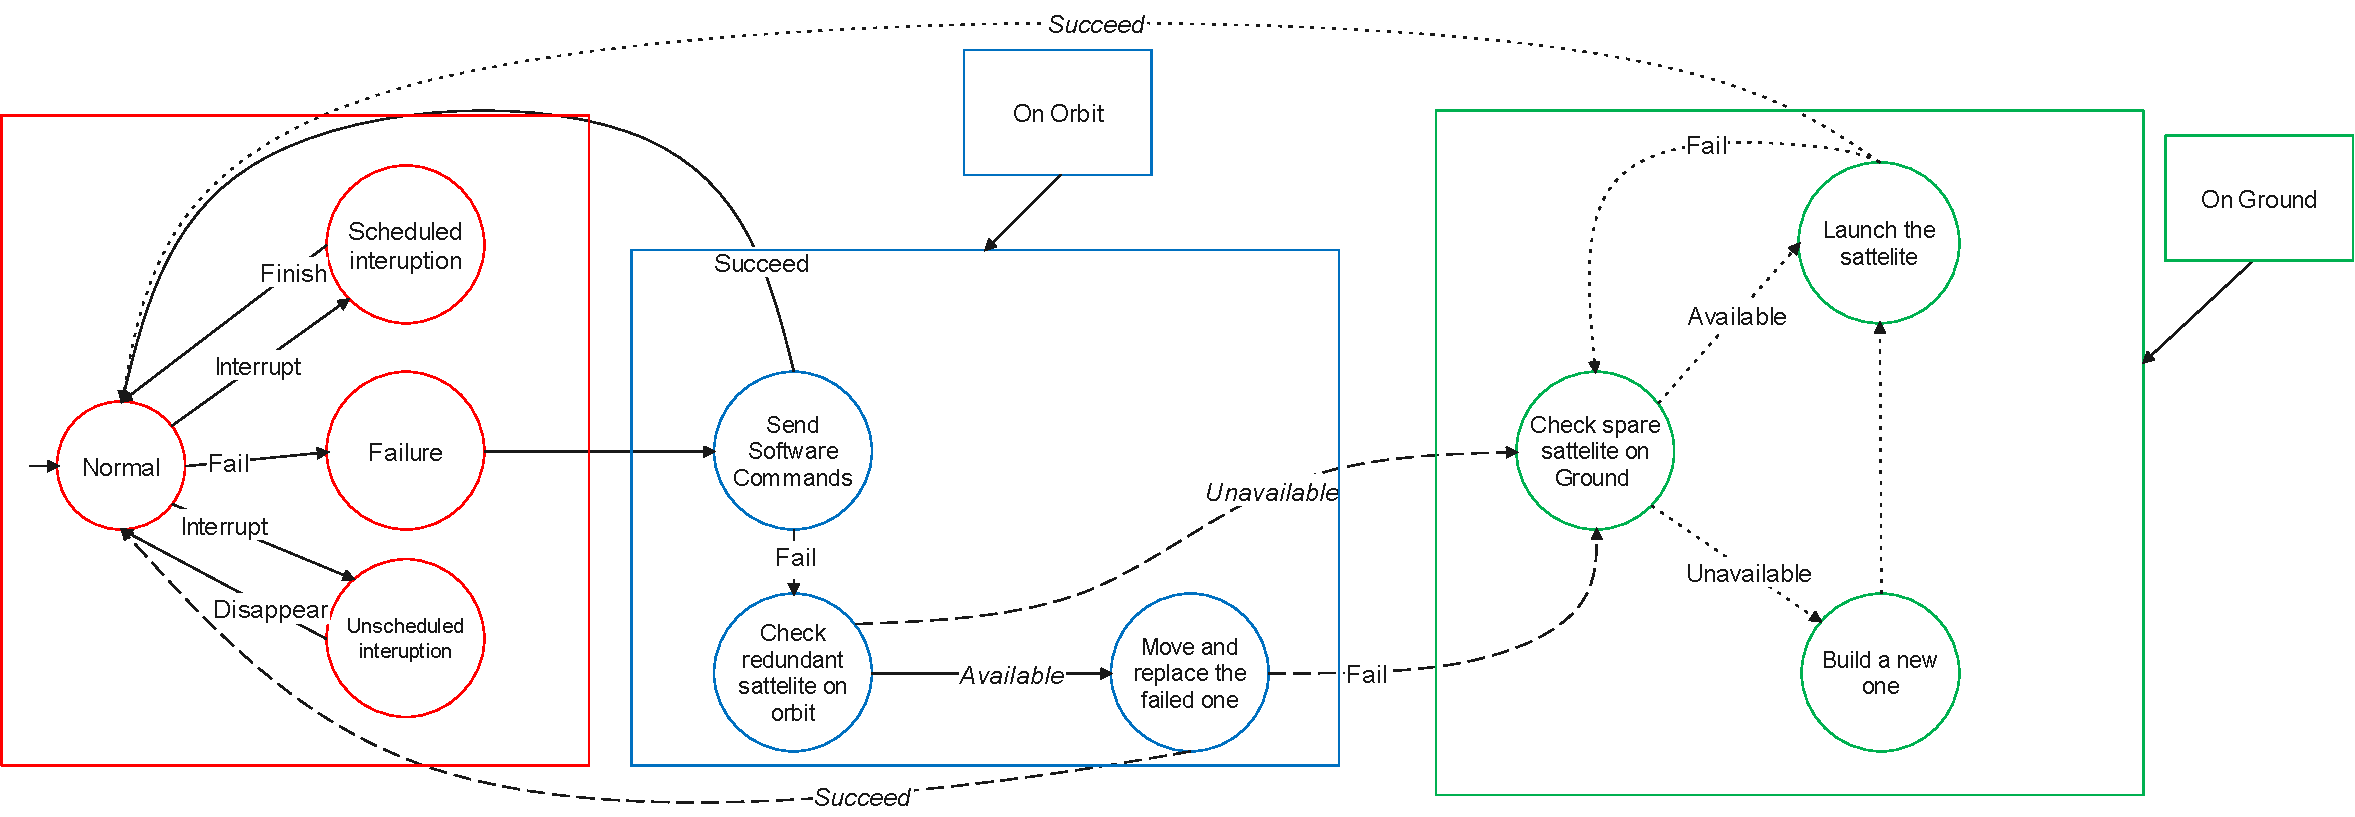
\includegraphics[width=500pt, height =180pt]{Dessin1.pdf}
    \caption{Satellite Maintenance Process Model \cite{Hoque2015,Yu2015}}
    \label{fig:usecase}
\end{figure*} 

\subsection{The system model}
This paper leverages a previously established satellite model described in \cite{Hoque2015,Yu2015,Zhaoguang2013}. The model considers the system's vulnerability to both scheduled and unscheduled interruptions throughout its lifecycle. Scheduled interruptions occur due to maintenance or software updates, leading to temporary signal unavailability for a fixed duration of \emath{t_{\alpha}=}4,320 hours. Unscheduled interruptions, such as those caused by solar radiation, can induce a Single Event Upset (SEU) in the satellite's signal. Unlike scheduled events, SEUs are unpredictable but also self-correcting, resolving automatically. Permanent failures, however, necessitate maneuvers in orbit or on the ground.


Upon satellite failure, ground and orbit control evaluate the best course of action. In some cases, the issue might be resolved remotely by sending software commands to the satellite. If the problem persists, deploying a redundant satellite from orbit as a replacement may be necessary. However, if no backup satellite is available, a new one will need to be manufactured and launched, introducing the risk of a launch failure.

The probability of a satellite failure is \emath{1-r}, where \emath{r} is its reliability calculated from the failure rate and Mean Time Between Failures (MTBF). Both the unscheduled and scheduled interruption times are \emath{t_{\alpha} = 4320 h}. If a failure occurs, there is an \emath{p_{\beta}=80\%} chance of resolving it on orbit by replacing the faulty satellite with a redundant one. If on-orbit repair is impossible, a new satellite needs to be built. The ground control team manages this process. \cmt{The times taken to decide to build a new satellite and for one to be manufactured are} \emath{t_{\gamma}=24}  hours and \emath{t_{\delta}=24}, respectively. Following a successful launch with \emath{p_{n} =90\%}, it takes another  \emath{t_{k}=24} hours for the new satellite to reach its operational position.


\subsection{On orbit and ground support capabilities}
\label{humanlabel}


The modeled system involves multiple state transitions driven by the \emph{environment}, \emph{on-orbit staff}, and \emph{ground staff}. Each group performs specific tasks:
\begin{itemize}
	\item \emph{Environment}: Triggers scheduled, unscheduled, and failure events (represented by the environment player, denoted as \emath{\mathcal{P}_{env}}) shown in red in \fig{fig:usecase}. Their actions are labeled as \emath{\alpha}.
	\item  \emph{On-Orbit Staff}: These personnel (represented by  \emath{\mathcal{P}_{o})} handle tasks like sending commands, updating software, and maneuvering the satellite into the position shown in blue in \fig{fig:usecase}. Their actions are labeled as \emath{\beta}.
	\item \emph{On-Ground Staff}:  The ground control team (represented by\emath{\mathcal{P}_{g}}) is responsible for monitoring satellite health, building new satellites when necessary, and performing launches (shown in green in \fig{fig:usecase}). Their actions are labeled as \emath{\omega}.
\end{itemize}


To model composability, we introduce a dedicated PRISM module that acts as a non-player. This module encapsulates the environment, on-orbit actions, on-ground actions, and the PRISM commands needed to synchronize their interactions. We define a CSG model, G, as a game modeling the parallel composition of the environment player \emath{\mathcal{P}_{env}}, on-orbit staff player \emath{\mathcal{P}_{o}}, and ground staff player \emath{\mathcal{P}_{g}}. This composition is coordinated by the non-player model \emath{\mathcal{P}_{\mathcal{R}}.}


\begin{mydef} \label{def:csg} \normalfont A concurrent stochastic game (CSG) for reasoning on Sattelite system maintenance is a tuple \emath{G =\gl{N, S, \bar{S}, A, \delta, AP, L}}:

\begin{itemize}
	\item \emath{N =\{\mathcal{P}_{env},\mathcal{P}_{o}, \mathcal{P}_{g}\}} is a finite set of players,

 	\item \emath{S=S_{env} \times S_{o} \times S_{g}} is a set of states, where \emath{S_{env}}, \emath{S_{o}}, and \emath{S_{g}} are states controlled by the system model, the environment model \emath{\mathcal{P}_{env}}, the on-orbit player model \emath{\mathcal{P}_{o}}, and on-ground model \emath{\mathcal{P}_{g}}, respectively \emath{\cmt{(S_{env} \cap  S_{o} \cap S_{g} =\emptyset)},}
    and \emath{\bar{S} \subseteq S } is a set of initial states,


	 \item \emath{A= A_{env} \times A_{o} \times A_{g} } where \emath{A_{env}},  \emath{A_{o},} and \emath{A_{g}} are the actions available to the environment model, on-orbit model, and the on-ground model, respectively,
    \item \emath{\delta : S \times A \longrightarrow Dist(S)} is a probabilistic transition function. Each player \cmt{\emath{\mathcal{P}_{env},\mathcal{P}_{o}, \mathcal{P}_{g}}} selects an action \emath{\alpha,\beta,\omega}, the state of the game is updated according to the distribution \emath{\delta(s, (\alpha,\beta,\omega)) \in Dist(S),} 

    \item \emath{AP} is a subset of all predicates that can be built over state variables. AP includes:
    \begin{itemize}
	\item \emath{goal}, achieved when a successful operation is reached.
     \end{itemize}
    \item \emath{L: S \longrightarrow 2^{AP}} is a labeling function that assigns each state  \emath{s \in S}  to a set of atomic propositions (\emath{AP}).
\end{itemize}
\end{mydef}


Following the definition of the CSG players, The non-player commands of \emath{\mathcal{P}_{\mathcal{R}}} that record the strategy of the CSGs model are expressed through the following transition: \emath{s_m\gparrow{\alpha,\beta,\omega}s'_m}, where \emath{\alpha} represents the label of the environment commands, \emath{\beta} denotes the on-orbit command, and \emath{\omega} denotes the on-ground commands. The non-player is modeled by the operation semantics rules \ref{s1} and \ref{s2}. The \ref{s1} is achieved by composing the modules \emath{\mathcal{P}_{env}}, \ \emath{\mathcal{P}_{o}}, and \emath{\mathcal{P}_{g}.} The \emph{standby} action refers to the idle position of the player in the CSG model. In this composition, the probability of achieving on-orbit or on-grounds tasks is determined by \cmt{\emath{\prod_{i=1}^{|N|} \lambda_{i}} such that \emath{\lambda_{i} \in \mathbb{R}}}.


\begin{figure*}[th]
\begin{boxD}
%\framedtext{
	      \begin{equation}\label{s1} \frac{ \sset{\mathcal{P}_{env}}= s_{i}\gparrow{\alpha}_{\lambda_{1}}s'_{i}  \bigwedge_{j=0}^{|A_{o}|}  \sset{\mathcal{P}_{o}}= s_{j} \gparrow{\beta_{j}}_{\lambda_{2}}s'_{j}  \wedge
       \sset{\mathcal{P}_{g}}= s_{k}\gparrow{\omega}_{\lambda_{3}} s'_{k} 
       \wedge
         \sset{\mathcal{P}_{\mathcal{R}}}= s_{m}\gparrow{\alpha,\beta,\omega}s'_{m}
       } {  \langle s_{i},\ldots,s_{j},\ldots s_{k}, \ldots s_{m},\theta\rangle  \xrightarrow{\alpha,\beta,\omega}_{\lambda_{1} \cdot \lambda_{2} \cdot \lambda_{3}}\langle s'_{i},\ldots,s'_{j},\ldots,s'_{k},\ldots,s'_{m},\theta'\rangle } \tag{\emph{On-Orbit}} \end{equation} where \emath{\alpha = Fail \wedge \omega= standby}
 
	     \begin{equation}\label{s2} \frac{ \sset{\mathcal{P}_{env}}= s_{i}\gparrow{\alpha}_{\lambda_{1}}s'_{i} \wedge \sset{\mathcal{P}_{o}}= s_{j} \gparrow{\beta}_{\lambda_{2}}s'_{j} \bigwedge_{k=0}^{|A_{g}|} 
       \sset{\mathcal{P}_{g}}= s_{k}\gparrow{\omega_{k}}_{\lambda_{3}} s'_{k} 
       \wedge
         \sset{\mathcal{P}_{\mathcal{R}}}= s_{m}\gparrow{\alpha,\beta,\omega}s'_{m} 
       } {  \langle s_{i},\ldots,s_{j},\ldots s_{k}, \ldots s_{m},\theta\rangle  \xrightarrow{\alpha,\beta,\omega}_{\lambda_{1} \cdot \lambda_{2} \cdot \lambda_{3}}\langle s'_{i},\ldots,s'_{j},\ldots,s'_{k},\ldots,s'_{m},\theta'\rangle}  \tag{\emph{On-Ground}} \end{equation} where \emath{\alpha = Fail \wedge \beta= standby}
\end{boxD}
\label{op:sec}
 \caption{Operational Semantics Rules of the CSG Game Model.}
\end{figure*}


\subsection{Measure the efficacy of collaborative maneuvers}
Measuring the efficacy of collaborative maneuvers consists of synthesizing a strategy for players \emath{\mathcal{P}_{env}}, \emath{\mathcal{P}_{o}}, and \emath{\mathcal{P}_{g}} that has the objective of reaching a state-satisfying goal and maximizes the value of the reward. The specification for the synthesis of such strategy is given as rPATL property following the pattern \emath{\mathtt{  \langle\langle\textcolor{red}{\mathcal{P}_{env}}, \textcolor{red}{\mathcal{P}_{o}}, \textcolor{red}{\mathcal{P}_{g}}\rangle\rangle} \mathtt{ P=? [ F} \ goal\mathtt{]}} where \emath{goal=(}\quot{\emath{\textcolor{red}{win}}}\emath{\& \ \textcolor{red}{rounds}<=\textcolor{red}{k})} to quantitatively evaluate the efficacy of collaborative maneuvers to the round \emath{k}. However, to calculate the reward or cost related to collaborative maneuvers it will take the following pattern: \emath{\mathtt{  \langle\langle\textcolor{red}{\mathcal{P}_{env}}, \textcolor{red}{\mathcal{P}_{o}}, \textcolor{red}{\mathcal{P}_{g}}\rangle\rangle}} \emath{\mathtt{R\{}}\quot{\textcolor{red}{win}}\emath{{\}=?[F } \ goal\mathtt{]}} where \emath{goal} =(\emath{\textcolor{red}{rounds}<=\textcolor{red}{k}}). In this case, the reward reflects the number of times the collaborative maneuvers wins the game within a specific round  \emath{k.}
\end{sloppypar}

\section{Quantitative analysis using PRISM-games}\label{useCase}
\label{sec:useCase}
\begin{sloppypar}
The PRISM tool can evaluate a wide range of dependability properties. In this work, we are particularly interested in evaluating signal transmission performance, specifically focusing on scenarios where the individual experiencing distress maintains a good psychological status. The source code of our artifacts is available in \cite{newcas2025}.

	    \begin{resp}{\textbf{\textit{Property}}}
        \begin{equation}
        \label{eq1}\tag{Rescue}
         \mathtt{ P=? [ (s=\quot{\textcolor{red}{Rescued} }) \  U^{\leq T} \ !(s=\quot{\textcolor{red}{Rescued} })  ]} 
        \end{equation}
        \end{resp}
        \normalsize
        
In Property \ref{eq1}, we evaluate signal performance by calculating the probability that the satellite successfully collects the signal from a beacon, transmits it through FLS services, initiates an RLM request, alerts a rescue coordination center, and ultimately ensures the correct provision of RLS services. The label \quot{\textcolor{red}{\emathtt{Rescued}}} refers to the state where the satellite collects the signal sent by the person in distress. This successful rescue scenario requires the conjunction of several conditions to be met: 
\begin{enumerate}
\item The detection performance must be in the nominal state (\emathtt{SAR\_DETECTION\_S \geq Nominal}).
\item The FLS status must be nominal (\emathtt{SAR\_FLS\_S \geq Nominal}).
\item The RLS service must also be in a nominal state (\emathtt{SAR\_RLS\_S \geq Nominal}).
\end{enumerate}

\noindent
    \begin{figure}[!htb]
    \centering
       \begin{tabularx}{\linewidth}{ m{8cm} }
           
\noindent
 \begin{minipage}[t]{8cm}
     \centering

    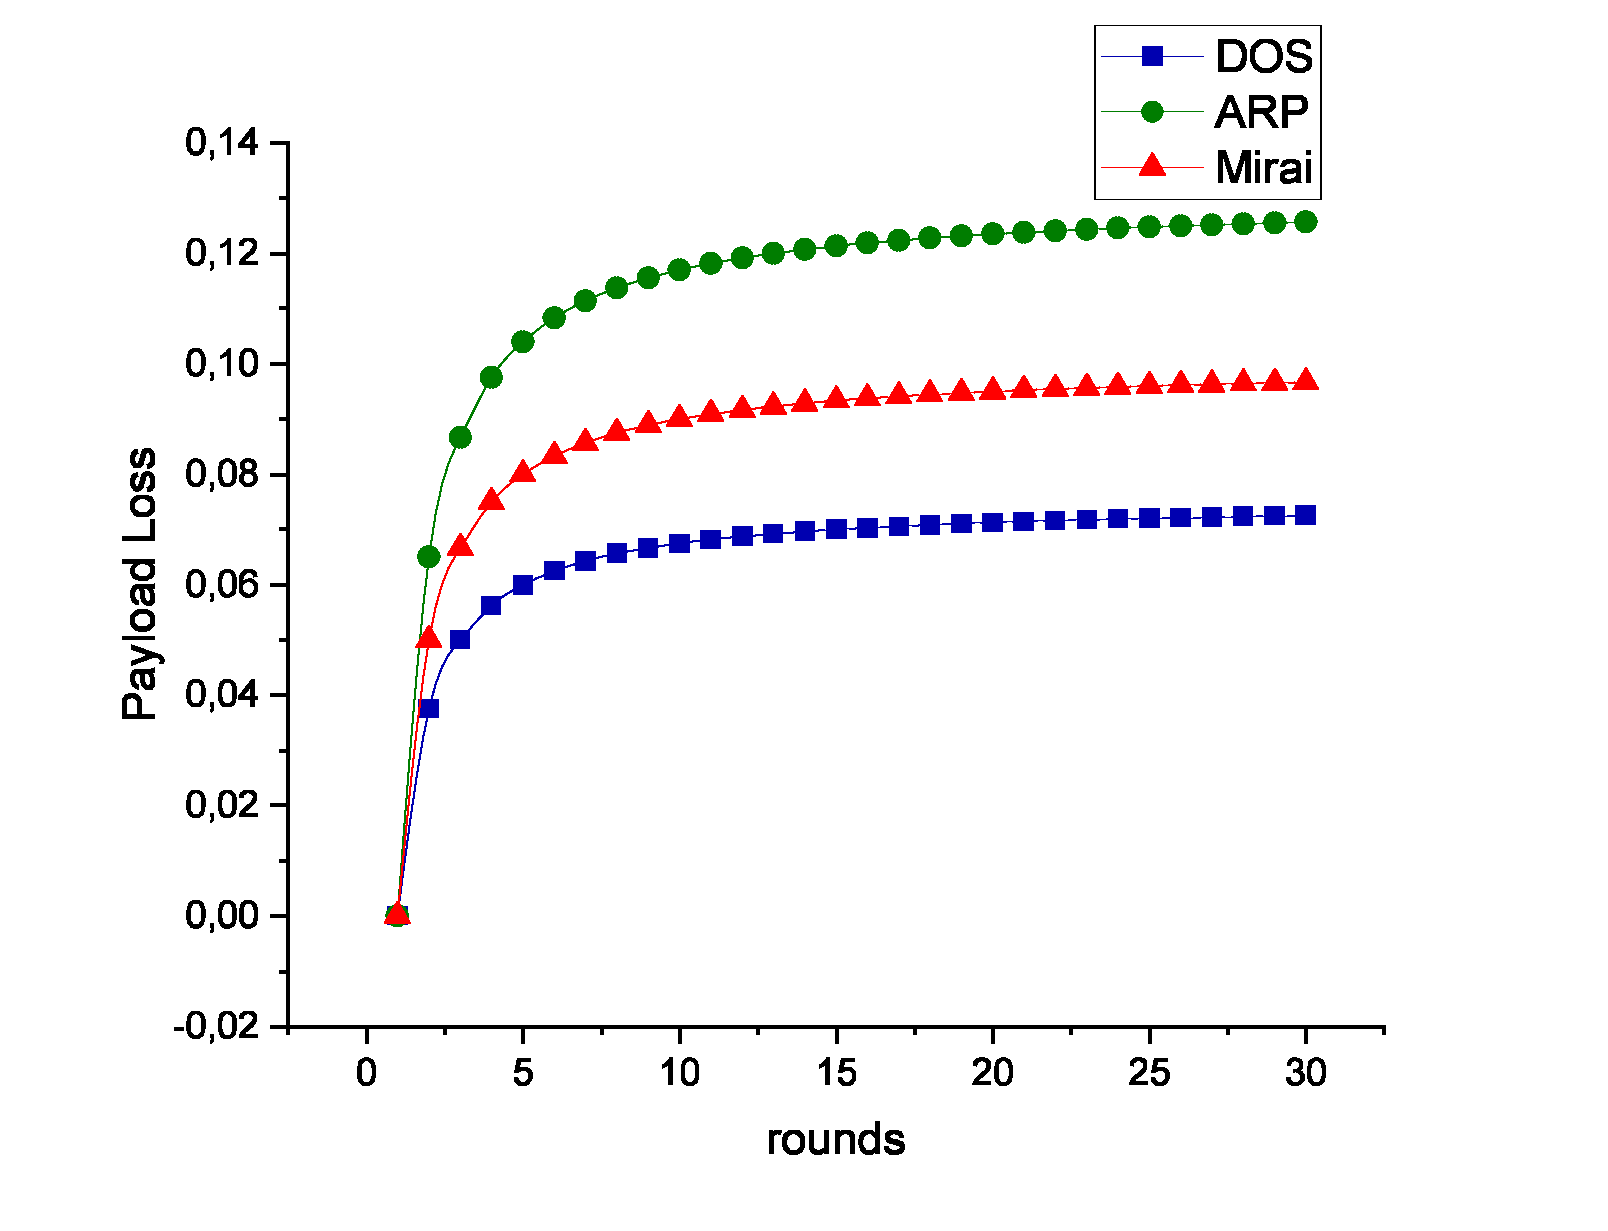
\includegraphics[width=250pt, height =180pt]{Graph2.pdf}
    \caption{Verification of Property \ref{eq1}.}
    \label{fig:01}
   \end{minipage}
    
          \\
\noindent
   \begin{minipage}[t]{8cm}
     \centering
   		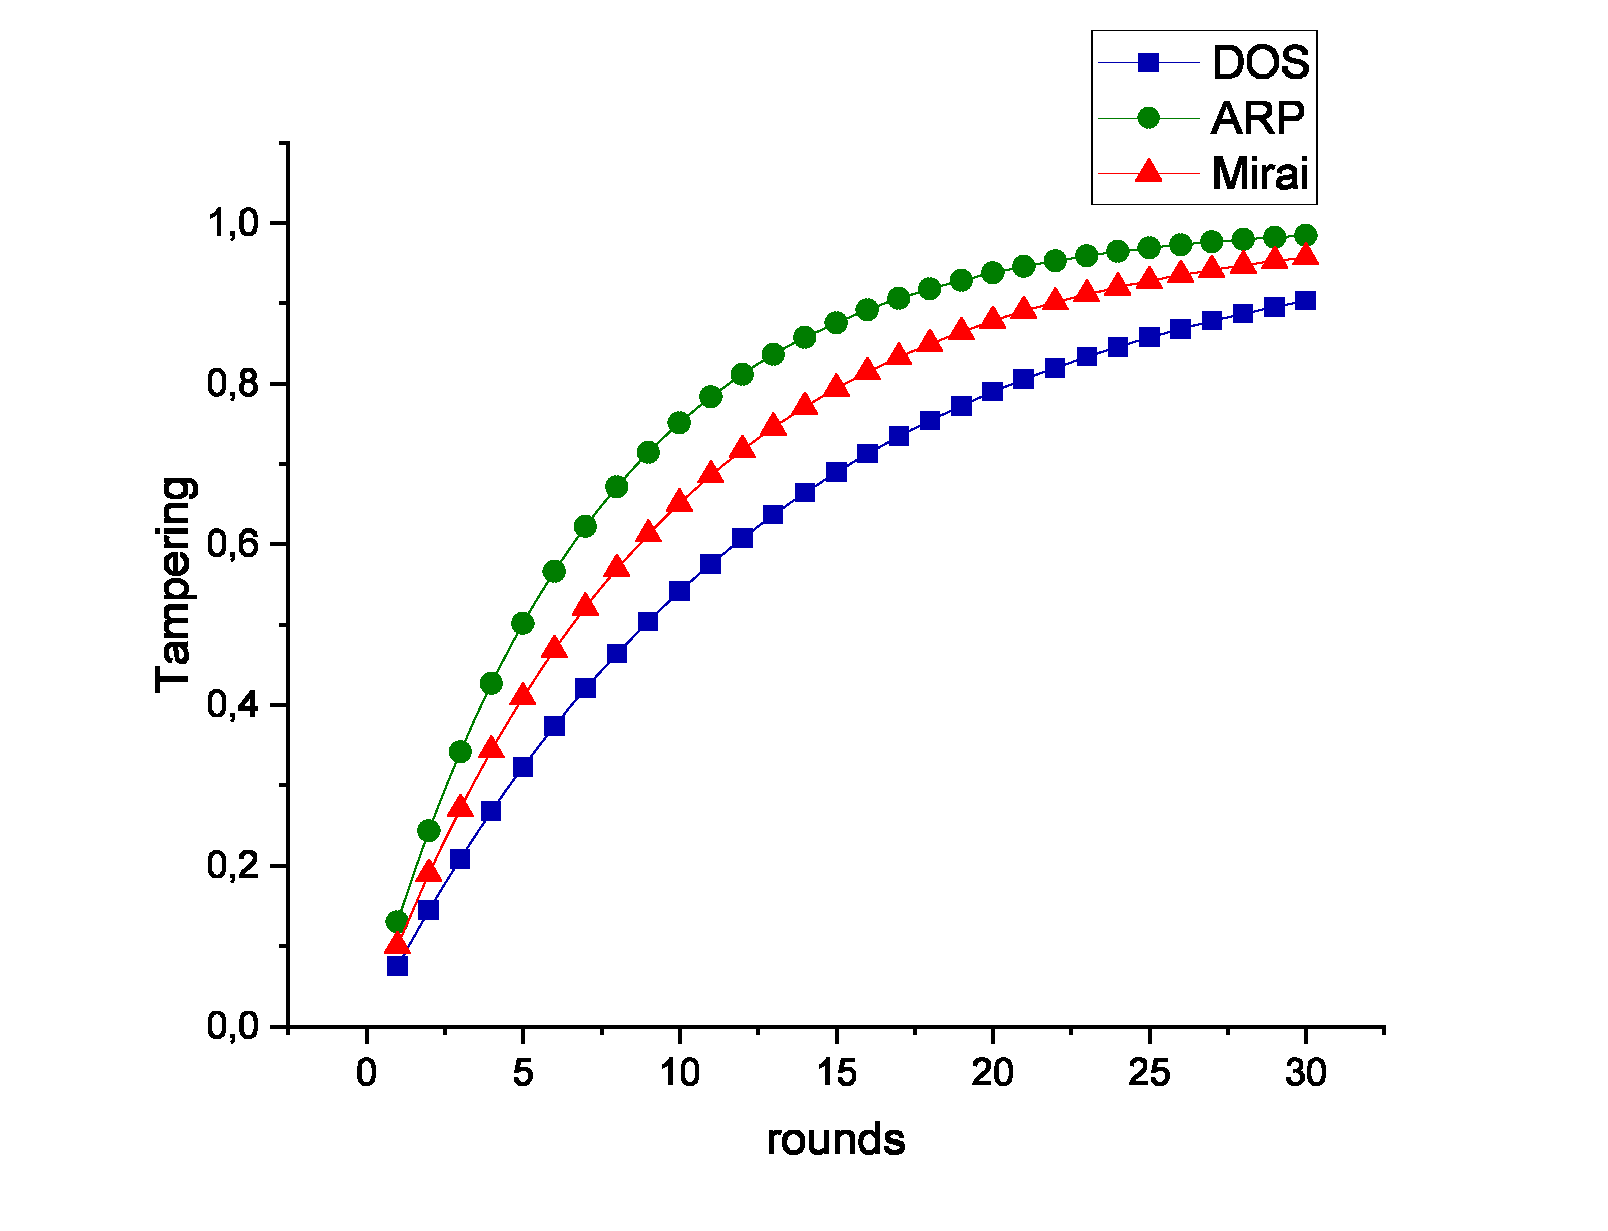
\includegraphics[width=250pt, height =180pt]{Graph1.pdf}
    \caption{Verification of Property \ref{eq1} wit MTTR.}
    \label{fig:02}
   \end{minipage}

               \end{tabularx}
\end{figure}

The results of verifying Property \ref{eq1} are depicted in Figure \fig{fig:01}. The system's ability to rescue the person decreases as time progresses. This is expected, as the SAR/Galileo service may not be able to effectively respond to the distress situation over longer durations. Figure \fig{fig:01} illustrates this system degradation over a period of 0 to 1 hour. It is important to note that our modeling considers degradations that can be detected within a 24-hours.

These results do not demonstrate the possibility that the system does not fully encompass the state of the human in terms of their reaction to danger, such as the Mean  Time To React to danger (MTTR). To address this limitation, we augment the model with a module that represents the human's status in response to a crisis in a one-month calendar. This module incorporates a formula for the rate of urgent response: 

\begin{equation*}
\lambda_{h} = MTTR / Month 
\end{equation*}

So, the model is augmented by human behavior, as shown in \lst{exampleinprism}, and the label \quot{\textcolor{red}{\emathtt{Rescued}}} includes human ability degradation.

\lstdefinestyle{framed}
{
	frame=lrb,
	mathescape,
	numbers=left,
	belowcaptionskip=-1pt,
	xleftmargin=3.11em,
	xrightmargin=0.03cm,
	framexleftmargin=3em,
	framexrightmargin=0pt,
	framextopmargin=5pt,
	framexbottommargin=5pt,
	framesep=0pt,
	rulesep=0pt,
	numbers=left,
}

\lstset{
    breaklines=true,
    style=framed,
    escapeinside={<@}{@>},
    morekeywords={void, int, public, private, class, protected, submodules, network, connections, const, init, int, bool, double, module, rewards, endrewards, endmodule},
    basicstyle=\scriptsize\ttfamily,
    keywordstyle=\bfseries\color{blue},
    morecomment=[f][\color{green!70!black}][0]{/*},
    morecomment=[l][\color{green!30!black}]{//},
    label=queueemodel
}

\begin{figure}[!htb]
\begin{minipage}{9cm}
\begin{lstlisting}[style=framed,
	caption=The Human Status,
 	label=exampleinprism]
module Human_Status
    Human_Status_s : [0..3] init 3;
    [] Human_Status_s>0 -> lambda_h:(Human_Status_s'=Degraded); 
endmodule
\end{lstlisting}
\end{minipage}
\end{figure}

We observe that the system's ability to rescue the person in distress decreases as the MTTR increases (within time windows of T=0.5 and T=0.1 of \fig{fig:01}). While this may seem intuitive, the verification process mathematically confirms this observation. Furthermore, the results demonstrate that the system's effectiveness depends on its capability to rescue the person in danger and crucially relies on the person's timely response to the crisis.


\end{sloppypar}


\section{Conclusion}\label{conclusion}
\begin{sloppypar}
This paper presents an approach based on CTMCs to model the communication services of the SAR/Galileo system. The captured model incorporates multiple degradation scenarios related to the observed and monitored communication between satellite systems and ground stations. We leverage the PRISM model checker for quantitative analysis, considering availability parameters and the evolving status of the distressed person.


An evaluation assessed which degradation source contributes most significantly to system failures and reduced reliability. Multiple factors were investigated, including loss of communication with monitoring ground stations and monitored failures attributed to human causes or environmental factors (the documentation does not explicitly mention the accurate sources of failures). The results demonstrate that ground stations responsible for monitoring signals are the most active sources of failures. Also, an evaluation has been performed to assess the human's capability to react to the crisis in conjunction with the system status. The results demonstrate that the \cmt{system and human parameters significantly influence performance}. 

Future work will consider incorporating additional parameters, such as the number of workstations, and exploring the implications of other formalisms, such as stochastic games, for assessing the reliability of human behavior in distress situations. The extension will also involve a comparative analysis between statistical model checkers and probabilistic model checkers to investigate the size of the resulting models and the feasibility of model verification.
\end{sloppypar}

%\newpage
\bibliographystyle{unsrt}
{\scriptsize
\bibliography{references}}

\end{document}
\endinput
%%
%% End of file `sample-sigconf.tex'.